\documentclass{article}
\usepackage{tikz}
\usetikzlibrary{arrows.meta, positioning, calc}

\begin{document}

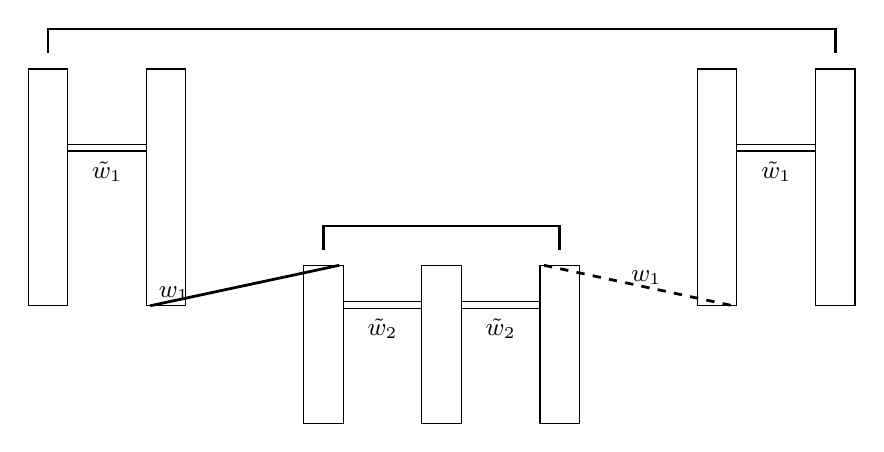
\begin{tikzpicture}[
    % Define styles for different line types
    double line/.style={double, double distance=2pt, line width=0.5pt},
    single line/.style={line width=1pt},
    dashed line/.style={dashed, line width=1pt},
    curved line/.style={line width=1pt, rounded corners=0pt},
    % Define block style
    block/.style={rectangle, draw, minimum width=0.5cm, minimum height=3cm},
    small block/.style={rectangle, draw, minimum width=0.5cm, minimum height=2cm},
    % Define label style
    label/.style={font=\small}
]

% First layer (top level)
\node[block] (b1) at (0,0) {};
\node[block] (b2) at (1.5,0) {};
\node[block] (b7) at (8.5,0) {};
\node[block] (b8) at (10,0) {};

% Second layer (bottom level)
\node[small block] (b3) at (3.5,-2) {};
\node[small block] (b4) at (5,-2) {};
\node[small block] (b5) at (6.5,-2) {};

% Double line connections (stride=1 convolutions)
\draw[double line] ($(b1.east)+(0,0.5)$) -- ($(b2.west)+(0,0.5)$);
\node[label] at ($(b1.east)!0.5!(b2.west)+(0,0.2)$) {$\tilde{w}_1$};

\draw[double line] ($(b4.east)+(0,0.5)$) -- ($(b5.west)+(0,0.5)$);
\node[label] at ($(b4.east)!0.5!(b5.west)+(0,0.2)$) {$\tilde{w}_2$};

\draw[double line] ($(b3.east)+(0,0.5)$) -- ($(b4.west)+(0,0.5)$);
\node[label] at ($(b3.east)!0.5!(b4.west)+(0,0.2)$) {$\tilde{w}_2$};

\draw[double line] ($(b7.east)+(0,0.5)$) -- ($(b8.west)+(0,0.5)$);
\node[label] at ($(b7.east)!0.5!(b8.west)+(0,0.2)$) {$\tilde{w}_1$};

% Single line connections (stride > 1 convolutions)
\draw[single line] ($(b2.south)-(0.2,0)$) -- ($(b3.north)+(0.2,0)$);
\node[label] at ($(b2.south)!0.3!(b3.north)-(0.5,0)$) {$w_1$};

% Dashed line connections (transpose convolutions)
\draw[dashed line] ($(b5.north)-(0.2,0)$) -- ($(b7.south)+(0.2,0)$);
\node[label] at ($(b5.north)!0.3!(b7.south)+(0.5,0)$) {$w_1$};

% Curved lines (skip connections)
\draw[curved line] 
    ($(b1.north)+(0,0.2)$) -- ($(b1.north)+(0,0.5)$) -- 
    ($(b8.north)+(0,0.5)$) -- ($(b8.north)+(0,0.2)$);

\draw[curved line] 
    ($(b3.north)+(0,0.2)$) -- ($(b3.north)+(0,0.5)$) -- 
    ($(b5.north)+(0,0.5)$) -- ($(b5.north)+(0,0.2)$);

\end{tikzpicture}

\end{document}